%%
%% Generated by gpt_translate from test/images.tex, on 2024-07-09 16:43:18 using model gpt-3.5-turbo-16k
%%

% GPT CHUNK%
\documentclass{ximera}
../preamble.tex
% 
% 'experimental' macro's, used over several files
% -> if useful -> move to preamble.tex
% -> else: remove ...

\usepackage{calculator} % gebruikt in goniomtrie/driehoeken om tangens te berekenen

\usepackage{eurosym}    % \euro  (€ werkt niet in xake ...?)

\usepackage{ulem} % \sout voor strike-out

% Nuttig als ook interactieve beamer slides worden voorzien:
\providecommand{\p}{} % default nothing ; potentially usefull for slides: redefine as \pause
%providecommand{\p}{\pause}

\usepackage{float}   % in binomiaalgetallen, om figure[H] in een uitweiding te krijgen; to be tested


\usepackage{caption} % captionof

\usepackage{pdflscape}    % landscape environment

\usetikzlibrary{matrix,decorations.pathreplacing,calc,fit,backgrounds}

% problem Metric TFM not found ... !\usepackage{esint} % various fancy integral symbols

% werkt niet :  (geeft missing $ of missing }  ... ????? )
%\def\oiint{\mathop{\vcenter{\mathchoice
%     {\huge\unicode{x222F}\,}{\unicode{x222F}}{\unicode{x222F}}{\unicode{x222F}}
%    }\,}\nolimits}

%\newcommand{\inlinechoiceoriginal}{\inlinechoice}
%
%
%\newcommand{\inlinechoicesquares}[2][]{%

%\newcommand{\dy}{\mathrm{d}y}
%\newcommand{\da}{\mathrm{d}a}
%\newcommand{\db}{\mathrm{d}b}
%\newcommand{\df}{\mathrm{d}f}
%\newcommand{\dg}{\mathrm{d}g}


%\pdfOnly{
%	\makeatletter
%	\setkeys{choice}{#1}%
%	\iffirstinlinechoice
%	%(\hspace{-.25em}
%	\firstinlinechoicefalse
%	\else
%	%/%
%	\fi
%	%\fbox{#2}
%	\ifthenelse{\boolean{\choice@correct}}%
%	{% Start then result
%		%\ifhandout\fbox{#2}\else\checkmark\ignorespaces\setkeys{choice}{correct=false}\ignorespaces\fi%
%		\ifhandout\fbox{#2\hphantom{\checkmark}}\else\fcolorbox{blue}{blue!20}{#2\checkmark}\ignorespaces\setkeys{choice}{correct=false}\ignorespaces\fi%
%	}% End then result
%	{% else
%		\fbox{#2\hphantom{\checkmark}}%	
%	}% Start/End else result
%	%\hspace{-.25em}\ignorespaces%
%	\makeatother
%}
%
%
%
%\newcommand{\setchoicesquares}{
%\ifdefined\HCode
%\else
%\renewenvironment{multipleChoice@}[1][]{}{}
%\renewcommand{\inlinechoice}[2][]{\inlinechoicesquares{}}
%\fi
%}
%
%\newcommand{\setchoiceinline}{
%	\ifdefined\HCode
%	\else
%	\renewenvironment{multipleChoice@}[1][]{}{)}
%	\renewcommand{\inlinechoice}{\inlinechoiceoriginal}
%	\fi
%}

\addPrintStyle{..}

\begin{document}
    \xmtitle{Images}{}

    \providecommand{\psize}[1]{
        \pgfmathparse{#1}
        \pgfmathresult pt
    }
    
    A tikzpicture without anything else:
        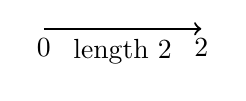
\begin{tikzpicture}
            \draw[thick,->]
            (0,0) node[below] {$0$} 
              --  node[below] {length 2}
            (2,0) node[below] {$2$};
        \end{tikzpicture}

    A tikzpicture inside a \verb|\begin{tikzpicture}[scale=2]|.
        \begin{tikzpicture}[scale=2]
            \draw[thick,->]
            (0,0) node[below] {$0$} 
              --  node[below] {length 2}
            (2,0) node[below] {$2$};
        \end{tikzpicture}

    A tikzpicture inside a \verb|\begin{tikzpicture}[scale=0.5]|.
        \begin{tikzpicture}[scale=0.5]
            \draw[thick,->]
            (0,0) node[above] {$0$} 
              --  node[below] {length 2}
            (2,0) node[above] {$2$};
        \end{tikzpicture}

 A tikzpicture inside a \verb|\begin{image}[1cm]| with size =\psize{1cm}.
    \begin{image}[1cm]
        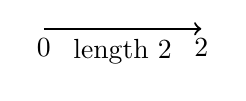
\begin{tikzpicture}
            \draw[thick,->]
            (0,0) node[below] {$0$} 
              --  node[below] {length 2}
            (2,0) node[below] {$2$};
        \end{tikzpicture}
    \end{image}

    A tikzpicture inside a \verb|\begin{image}[\textwidth]| with size =\psize{\textwidth} (and textwidth =\the\textwidth).

    \begin{image}[\textwidth]
        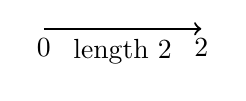
\begin{tikzpicture}
            \draw[thick,->]
            (0,0) node[below] {$0$} 
              --  node[below] {length 2}
            (2,0) node[below] {$2$};
        \end{tikzpicture}
    \end{image}

    A tikzpicture inside a \verb|\begin{image}[0.5\textwidth]| with size =\psize{0.5\textwidth}.
    \begin{image}[0.5\textwidth]
        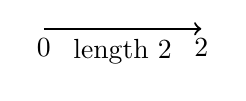
\begin{tikzpicture}
            \draw[thick,->]
            (0,0) node[below] {$0$} 
              --  node[below] {length 2}
            (2,0) node[below] {$2$};
        \end{tikzpicture}
    \end{image}

    A tikzpicture inside a \verb|\begin{image}[0.2\textwidth]| with size =\psize{0.2\textwidth}.
    \begin{image}[0.2\textwidth]
        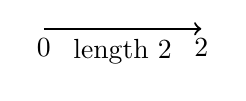
\begin{tikzpicture}
            \draw[thick,->]
            (0,0) node[below] {$0$} 
              --  node[below] {length 2}
            (2,0) node[below] {$2$};
        \end{tikzpicture}
    \end{image}

    A tikzpicture inside a \verb|\begin{image}[10cm]| with size =\psize{10cm}.
    \begin{image}[10cm]
        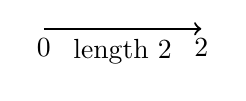
\begin{tikzpicture}
            \draw[thick,->]
            (0,0) node[below] {$0$} 
              --  node[below] {length 2}
            (2,0) node[below] {$2$};
        \end{tikzpicture}
    \end{image}

    A tikzpicture inside a \verb|\begin{image}[5cm]| with size =\psize{5cm}.
    \begin{image}[5cm]
        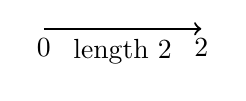
\begin{tikzpicture}
            \draw[thick,->]
            (0,0) node[below] {$0$} 
              --  node[below] {length 2}
            (2,0) node[below] {$2$};
        \end{tikzpicture}
    \end{image}

    A tikzpicture inside a \verb|\begin{image}[1cm]| with size =\psize{1cm}.
    \begin{image}[1cm]
        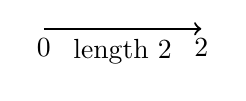
\begin{tikzpicture}
            \draw[thick,->]
            (0,0) node[below] {$0$} 
              --  node[below] {length 2}
            (2,0) node[below] {$2$};
        \end{tikzpicture}
    \end{image}

          

    \end{document}